\section{Markets for a Self-Incentivizing Network}
\label{sec:designs}
We set out to design a market interface that any router could expose and users could interact with multiple markets.
We wanted to allow different users with their own objectives to be able to buy guaruntees of packet carriage but also change their reservations to increase their own percieved utility.

In the rest of the section, we introduce a first simple market to achieve these goals and then evaluate its performance with simulated users.
This intial design has high overhead and our current simulated users have the ability to change their utility for the worse because of market races with other users. We quantify this phenomena with a worst case "evil user," and finally propose a new multi-resolution market that addresses these problems.

%\begin{itemize}
%
%\item Let anybody contribute capacity
%
%\item Allow users with different utility functions to interact (flow completion time vs.~jitter)
%
%\item Allow users to buy guarantees (and not get swindled)
%
%\end{itemize}

\subsection{Simple Market Design}
Our market is composed of consecutive time slots in which a single packet can be delivered. Users are able to buy the rights to deliver a packet at a given time slot for a reserve price set by the market. Once a slot is owned by a user, they have the right to send a packet on the link at that time if they can deliver a packet to the router before that time. They can also add an offer to the slot to re-sell it to another user if they pay the offer price. figref gives the basic market layout.

\begin{figure}
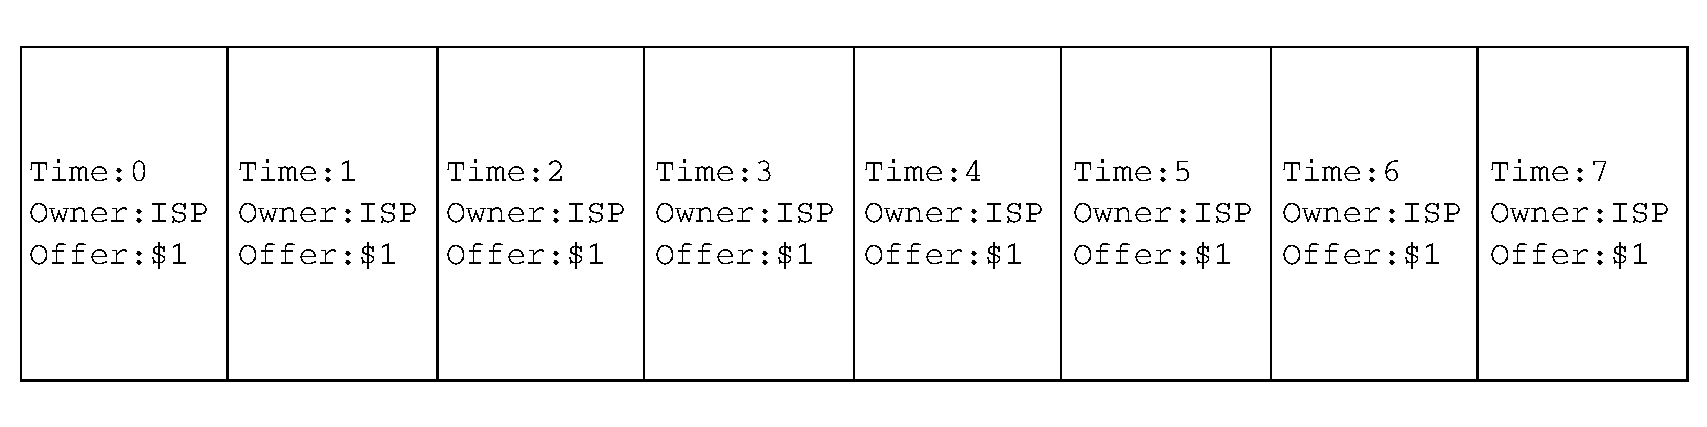
\includegraphics[width=\columnwidth]{diagrams/simple_market.pdf}
\caption{Simple market diagram}
\label{f:simple_market}
\end{figure}

\subsection{Simple Market Evaluation}

Simulation experiments to test whether the one-layer market has each desired property?

Measure outcome quality (vs.~SRTF or other optimal), \# of roundtrips

can simulate multiple users with different objectives

\begin{figure}
%\vspace{\baselineskip}
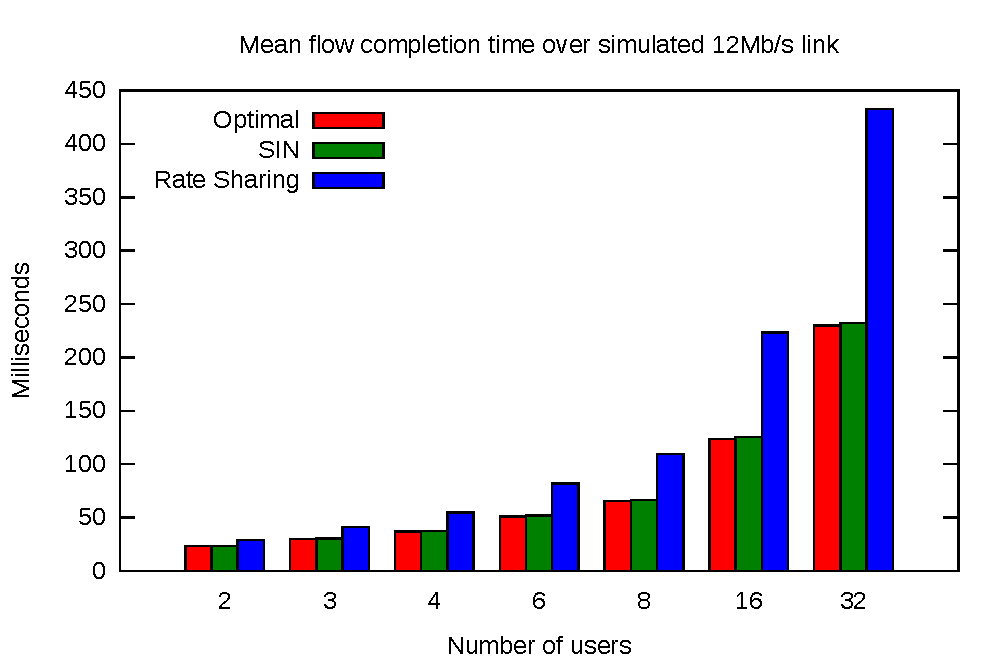
\includegraphics[width=\columnwidth]{plots/delay_over_srtf.pdf}
\caption{Average queuing delay of simlulations divided by the average queuing delay of the optimal shortest remaining time first solution.}
\label{f:delay_over_srtf}
\end{figure}

\begin{figure}
%\vspace{\baselineskip}
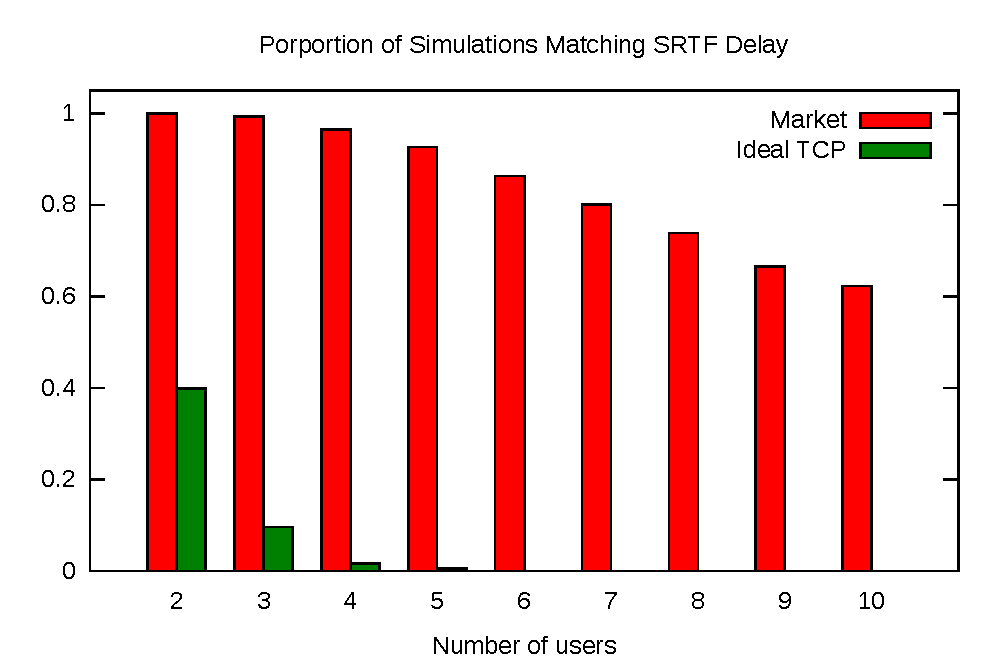
\includegraphics[width=\columnwidth]{plots/percent_match_srtf.pdf}
\caption{Percent of simlulations that achieved optimal shortest remaining time first solution.}
\label{f:percent_match_srtf}
\end{figure}

We simulated the results of running a market in practice with users that would arrive at time $t$ had a known number of packets $n$ they wanted to send.
Their utility is defined as:.
Figures~\ref{f:delay_over_srtf} and \ref{f:percent_match_srtf} show the result of running the simulation with 2 to 10 concurrent users, all trying to minimize their flow completion time for the cheapest cost.
We compare with a round robin scheme, which is the ideal equillibrium of mutliple TCP flows and a FIFO queued router (TODO cite).
In our simulations, there are a varying number of users with a flow start time chosen from a uniform random distribution between 0 and 9 with flow lengths chosen from a uniform random distribution between 1 and 10. We compare to the allocation of packets to times that minimizes the queued time for each flow: shortest remaining time first scheduling (TODO cite).

We find that bots in our market almost always converge on an allocation that is equivalent to the optimal shortest remaining time first schedule when there is a small number of users. Larger numbers of users are less likely to achieve an optimal solution, but the excess queuing delay over the optimal SRTF solution remains extremely low with a large number of users: less than 1\% overhead in all of our evaluations.

problem with current design, introduce evil user
problem: exposure problem, evil user

the problems we encountered with the simple market led us to our current design:
\subsection{Multi-Layer Market Design}

Sketch of multi-layer design
